\chapter{Conclusions and Future Work}
\label{sec:ch7}

The work shown throughout this document can also be found in Refs. \cite{cris1,cris2, cris3}. This section reports on the conclusions and future work stemming from this thesis.

\section{Conclusions}

\subsection{RDTs and Resonance Compensation}

The measurement and subsequent cancellation of RDTs was investigated in depth in Ch. \ref{sec:ch4}.

\subsection{Physics-Informed vs. Optimization-Based Compensation}

Chapters \ref{sec:ch4} and \ref{sec:ch5} showed two different approaches to the same problem of resonance compensation. The first one performed at the Fermilab Recycler Ring showed how to implement the response matrix approach, which can be traced to some underlying physics principles. On the other hand, Ch. \ref{sec:ch5} shows how to implement numerical optimization algorithms for compensating multiple resonance lines at the CERN PS Booster. Nevertheless, this last approach had no direct physics input. The distinction between a physics-informed approach and a numerical-optimization approach summarizes the differences between both chapters. 

\subsection{High-Intensity Resonance Compensation}

\subsection{Transverse Dampers and High-Intensity Compensation}

\begin{figure}[H]
    \centering
    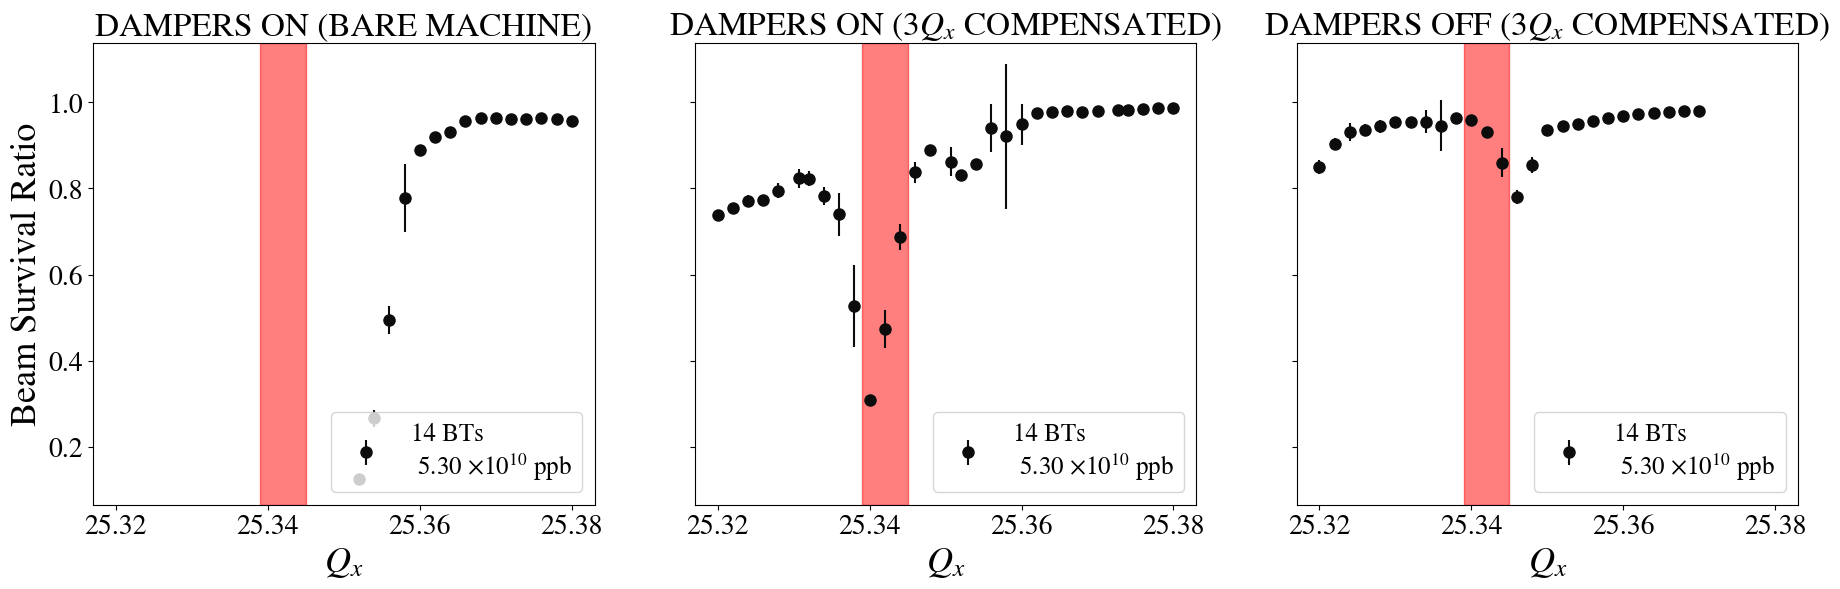
\includegraphics[width=\columnwidth]{chapter7/dampers_config.png}
    \caption{Transverse damper effect on resonance compensation for bare machine + dampers ON, $3Q_x$ compensated + dampers ON, and $3Q_x$ compensated + dampers OFF configuration. The red band corresponds to the $3Q_x$ stop band at an intensity of 0.5 ppb with dampers ON.}
    \label{fig:dampers7}
\end{figure}

\section{Future Work}

\subsection{Verification of Newly-Installed Sextupoles}

Section \ref{sec:compensate} explained the motivation behind installing additional sextupoles that would bring down that currents needed to compensate $3Q_x=76$ and $Q_x+ 2Q_y = 74$. Subsequently, Sec. \ref{sec:addsexts} explained the procedure used in order to pin down the new locations for two new compensation sextupoles. There is still future work to be done regarding the commissioning and connection of the new 620 sextupoles. The sextupoles and their power supplies need to be interfaced with ACNET. Furthermore, the resonance compensation enhancement still needs to verified by means of performing an RDT scan. Specifically, the response matrix coefficients corresponding to these new sextupoles need to be measured and calculated. All of this, following the procedure outlined in Secs. \ref{sec:rdtmeasure} and \ref{sec:compensate}.

\begin{figure}[H]
    \centering
    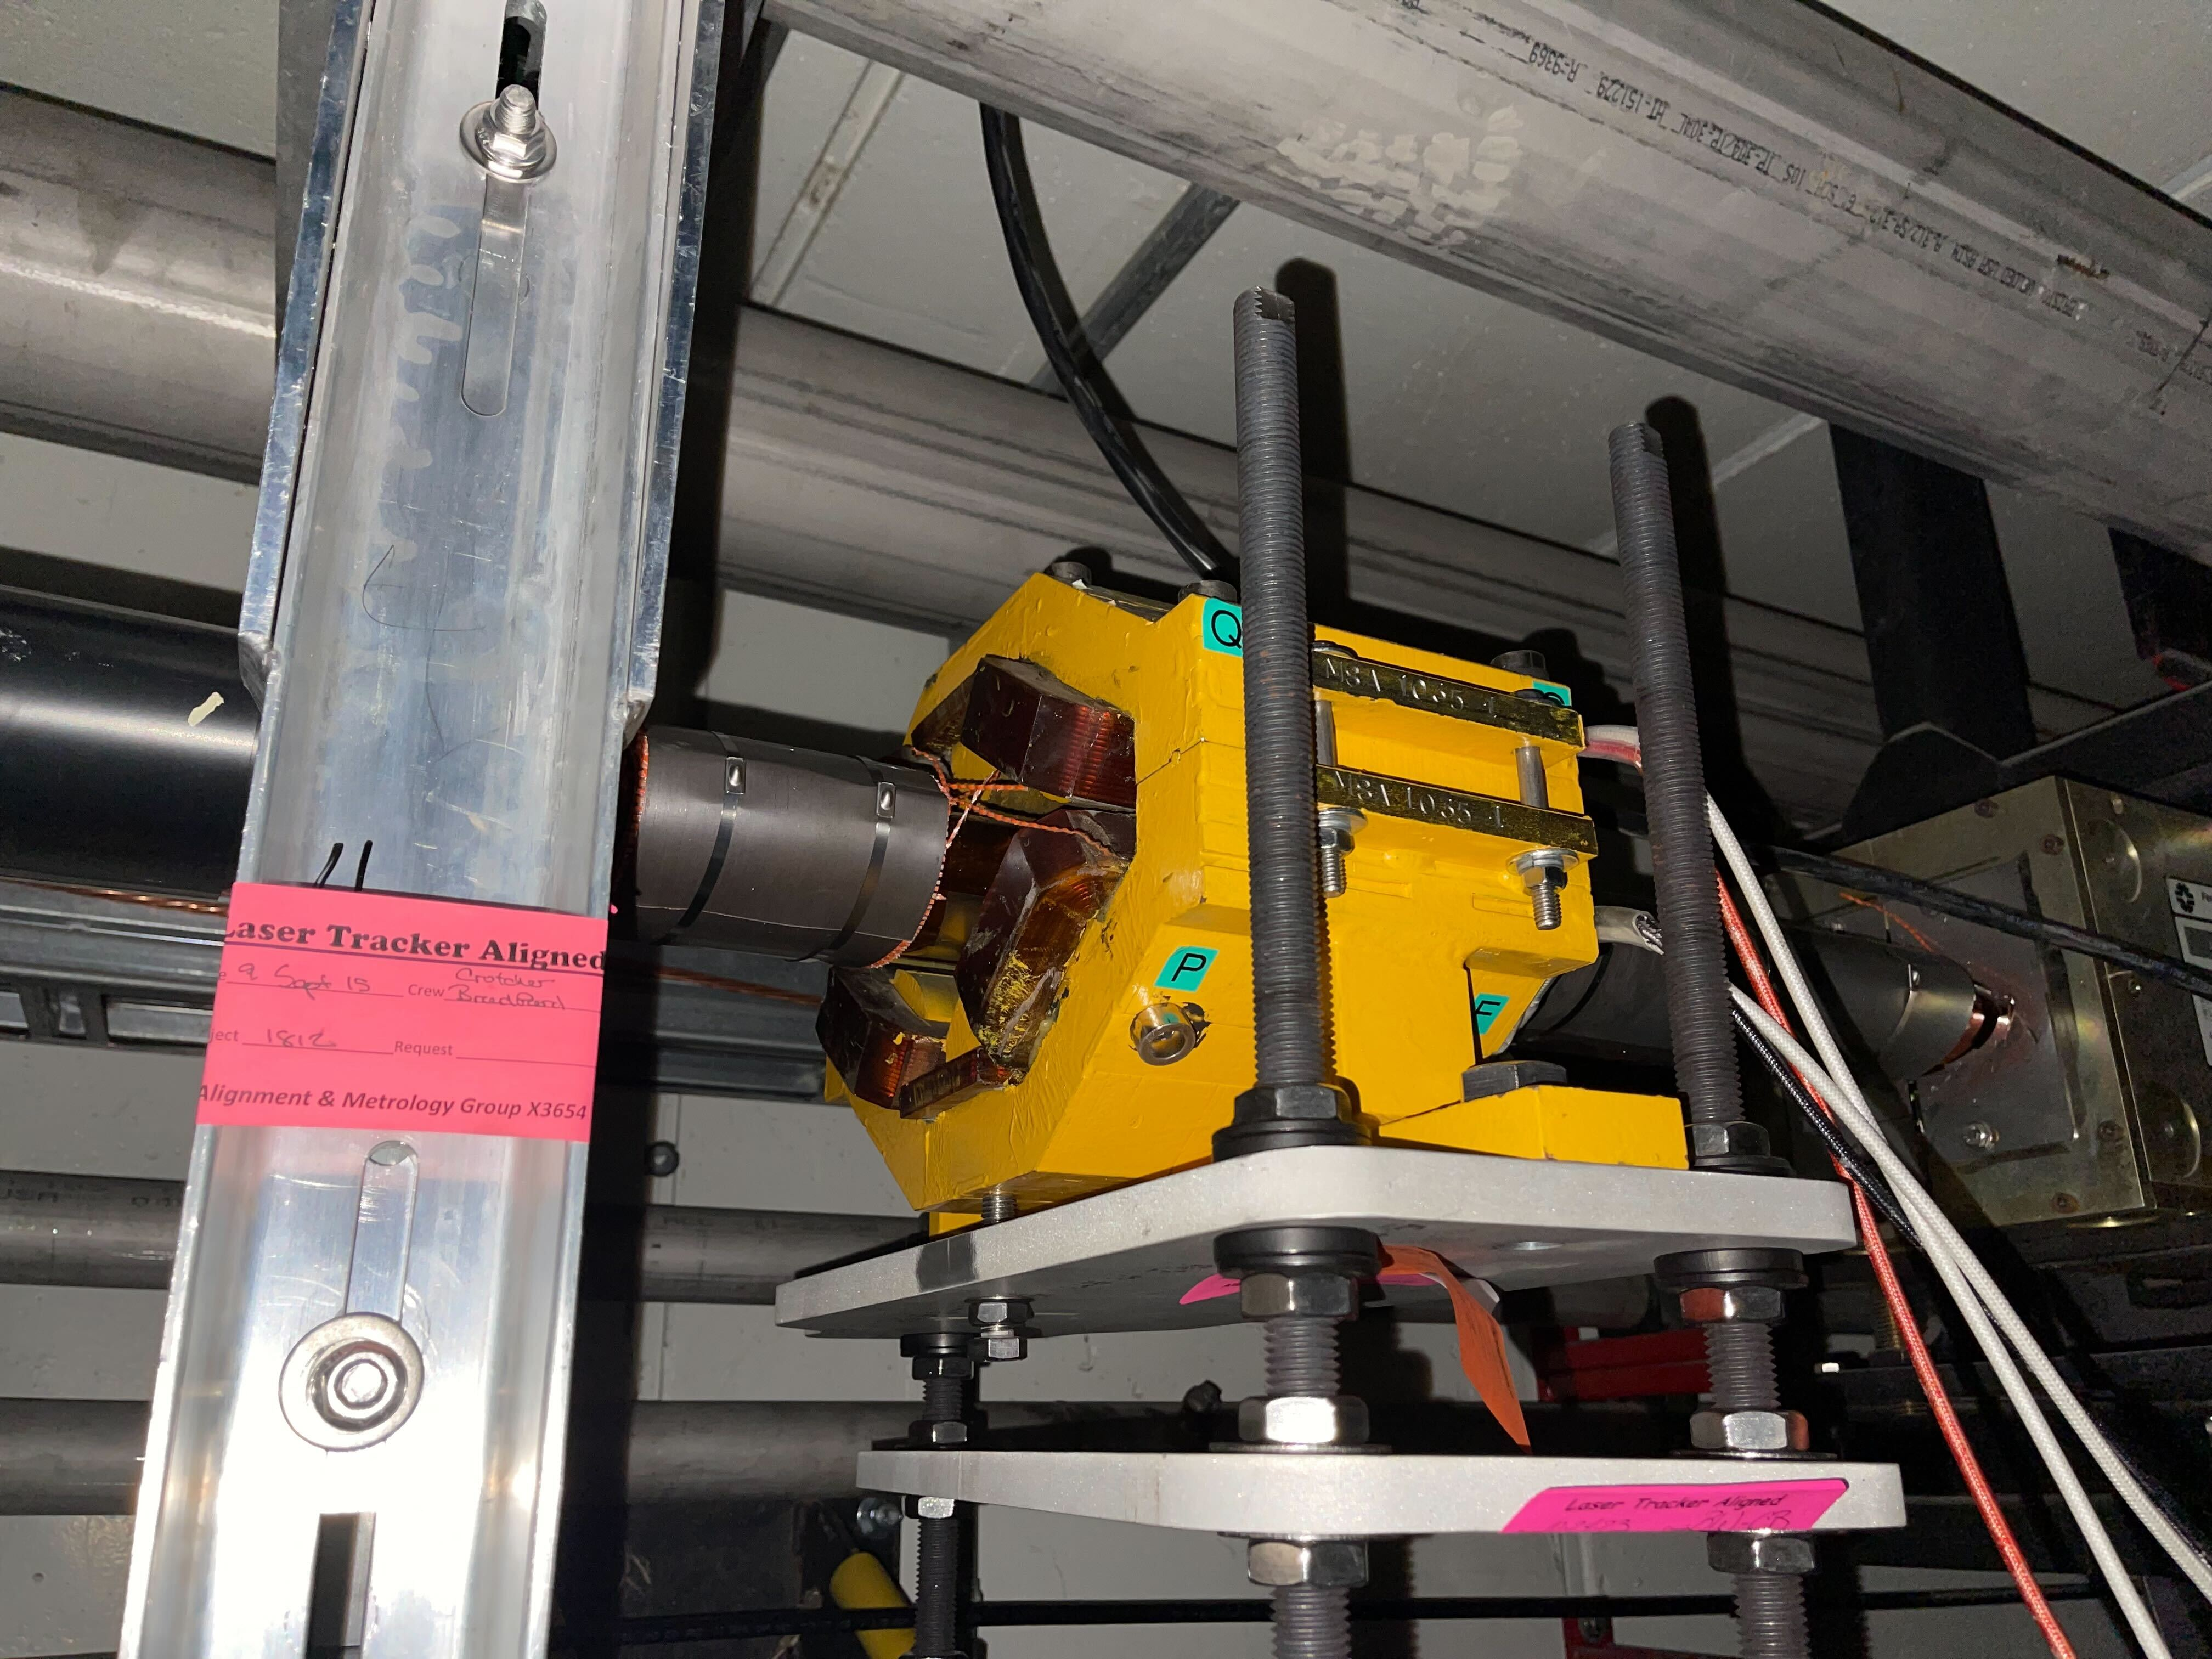
\includegraphics[width=\columnwidth]{chapter7/620_sext.jpg}
    \caption{Newly installed compensation sextupoles in the 620 section.}
    \label{fig:new620sexts}
\end{figure}

\subsection{Resonances and Transverse Dampers at High Intensities}


\subsection{Effect of MI Ramp on RDTs}

The ultimate objective of this work is to have this resonance compensation scheme fully characterized in order to incorporate it into high intensity operations. Nevertheless, there are two additional factors that have been identified to also play a role in this effort. The first one stems from the fact that the Main Injector and the Recycler Ring share the same tunnel. It has been shown that the acceleration ramp changes the beam dynamics inside the Recycler Ring. In particular, it introduces orbit distortions and tune shifts depending on the position of the ramp \cite{mionrr}. There is an ongoing effort in order to characterize any higher order magnetic effect from the MI to RR, e.g., any sextupole term that is being introduced by the MI acceleration ramp. The first results have shown that the compensation currents change depending on the location of the study event with respect to the MI acceleration ramp. Therefore, in the future, the resonance compensation described hereinabove should be modified to accommodate this effect to be fully operational.

\subsection{Limits of Resonance Compensation}

\subsection{Space Charge RDTs}
